\newif\ifQR
%\QRtrue
\QRfalse

\documentclass[uplatex,a4paper]{jsarticle}
\usepackage[at]{easylist} 
\usepackage{eclbkbox}
\usepackage[yyyymmdd]{datetime}
\usepackage{fancyhdr}
\usepackage{multicol}

\pagestyle{fancy}
\title{T51: Strategic Japanese: Particle 01 Task Sheet}
\author{Hilofumi Yamamoto}
\date{Tokyo Institute of Technology}
%\date{2018.04.19 Ookayama\hspace*{4em}2018.04.22 Suzukakedai}
\setlength{\topmargin}{-16mm}
\setlength{\textheight}{1.3\textheight}
\lhead{\jobname}
\chead{Strategic Japanese}
\rhead{\today\,\currenttime}
\usepackage[dvipdfmx]{graphicx}	% required for `\includegraphics' (yatex added)
\begin{document}
%\maketitle
\thispagestyle{fancy}

{\noindent\LARGE Strategic Japanese: Particle 1}

\vspace*{.5\baselineskip}

%{\noindent\large Hilofumi Yamamoto --- Tokyo Institute of Technology}

You can omit particles as much as you can.
But there are some cases you cannot ommit them.
Having said that, in that case you may omit a verb in that sentence instead of the particle.

\section{Model}

Please speak freely as natural as possible! 

\begin{flushright}
%\includegraphics[trim=40 70 70 190, clip, width=.45\hsize]{bus-nidewo.pdf}
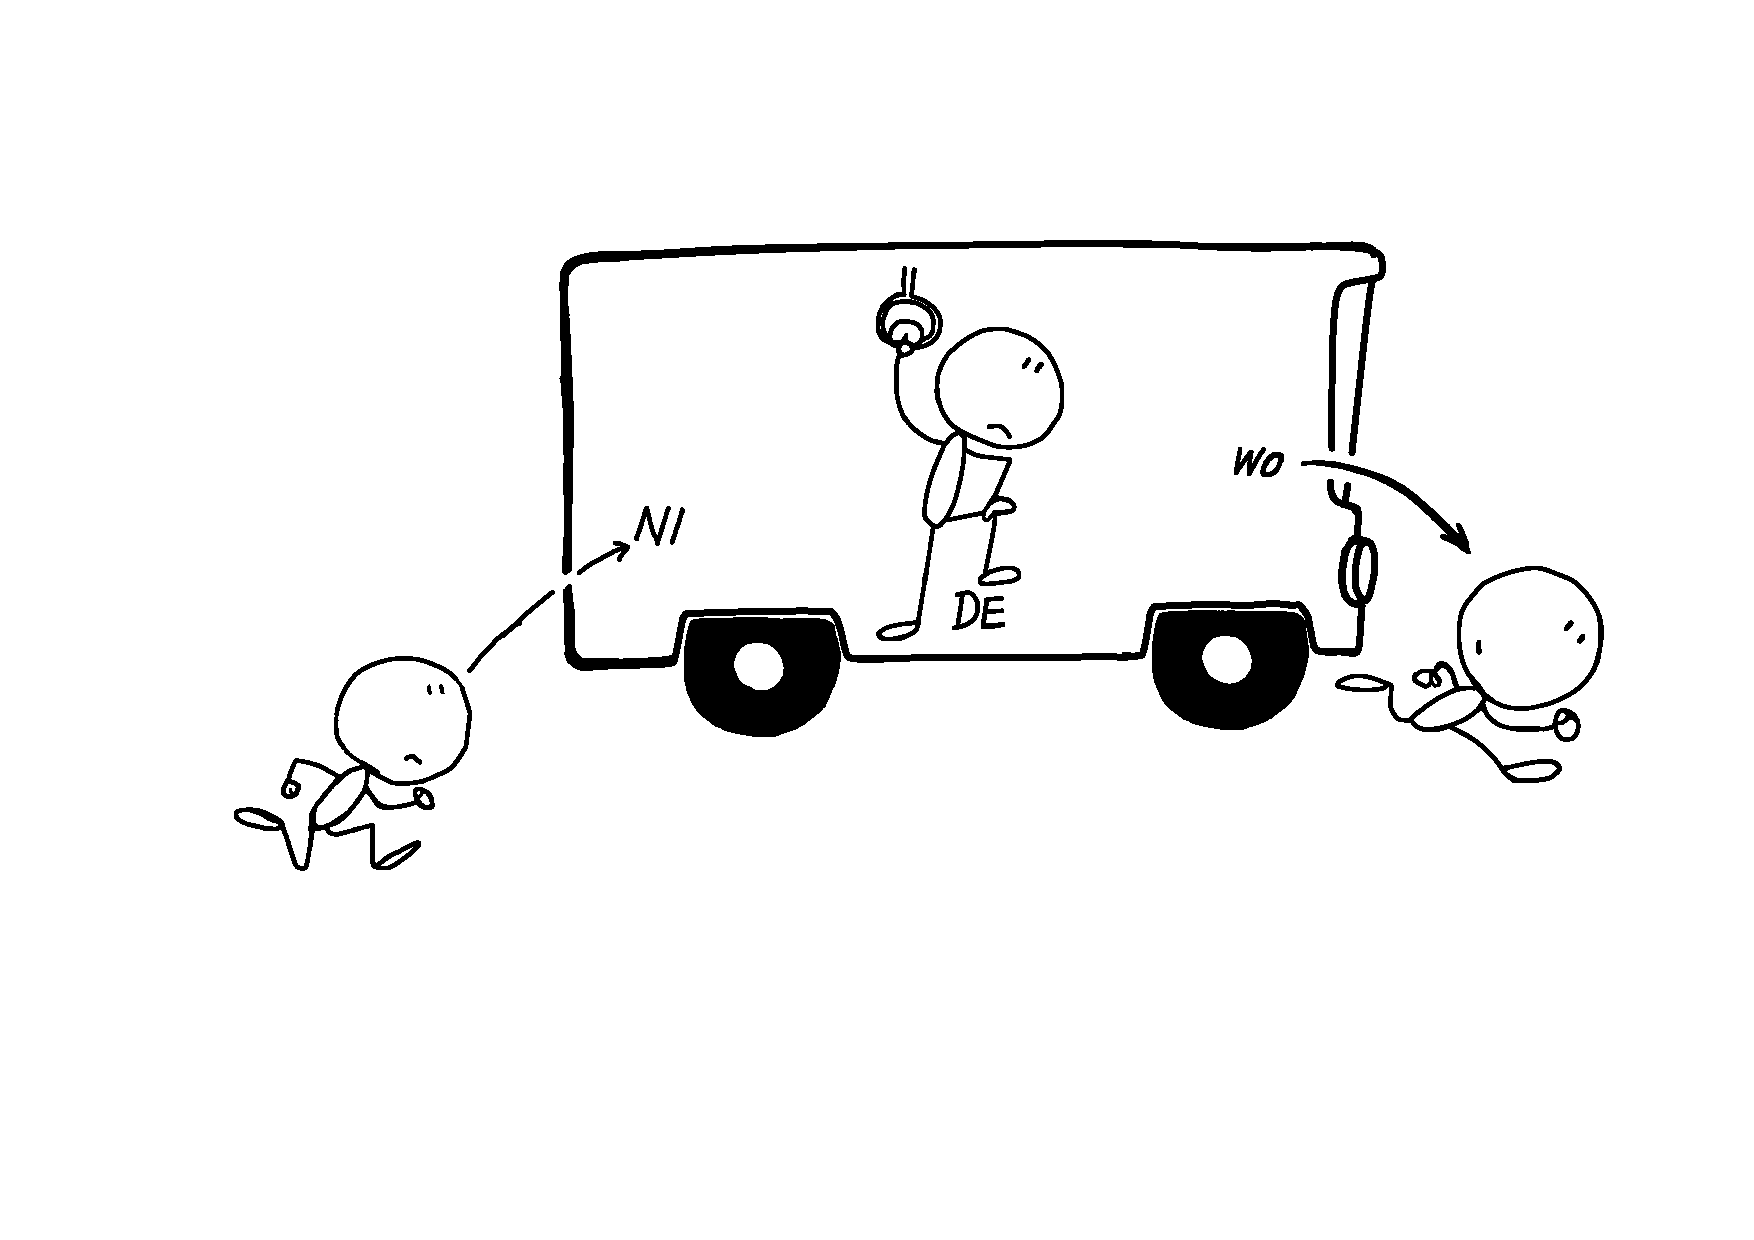
\includegraphics[trim=100 170 70 100, clip, width=.45\hsize]{2019-06-01.pdf}
\end{flushright}

\vspace*{-8\baselineskip}

\begin{itemize}
   \item[A:] Kinou doko itta? (Yesterday, where did you visit?) 
   \item[B:] Shibuya \underline{{\bfseries ni}} itta. (I went to Shibuya)
   \item[A:] Densha \underline{{\bfseries de}} itta? (Did you go by train?)
   \item[B:] Uun, basu \underline{{\bfseries de}}. (No, by bus)
   \item[A:] Densha \underline{{\bfseries ni}} notta? (Did you get on train?) 
   \item[B:] \underline{{\bfseries Uun, noranakatta.}} (No, I didn't)
\end{itemize}

%\vspace*{4\baselineskip}

\section{Task}
 
Convert the following verbs into past tense and negative past tense.

\begin{multicols}{2}
\begin{enumerate}
\setcounter{enumi}{-1}   
 \item  taberu (eat)  $\rightarrow$ \underline{\bfseries tabeta / tabenakatta\hspace{1em}}
 \item  miru (see)    $\rightarrow$ \hrulefill
 \item  yomu (read)   $\rightarrow$ \hrulefill
 \item  kaku (write)  $\rightarrow$ \hrulefill
 \item  tsukuru (make)$\rightarrow$ \hrulefill
 \item  iku  (go)     $\rightarrow$ \hrulefill
 \item  suru (do)     $\rightarrow$ \hrulefill
 \item  kuru (come)   $\rightarrow$ \hrulefill
\end{enumerate}
\end{multicols}

\section{Activity}

Ask your classmates in both casual and formal style.

\begin{multicols}{2}
\begin{itemize}
 \item[A:] a. \underline{ Suzuki } san, kinou doko itta?
 \item[A:] Nan {\bfseries de} itta? (How did you get there?)
 \item[B:] b. \underline{ {\bfseries Shibuya ni}} itta.
 \item[B:] c. \underline{ {\bfseries Basu de} }. (By bus)
\end{itemize}
\end{multicols}

\begin{enumerate}
\setcounter{enumi}{-1}   
 \item a. \underline{ Suzuki\hspace{6.4zw}}, b. \underline{ Shibuya\hspace{10.4zw}}, c. \underline{ basu\hspace{13.2zw}}.
 \item a. \underline{\hspace{10zw}}, b. \underline{\hspace{15zw}}, c. \hrulefill.
 \item a. \underline{\hspace{10zw}}, b. \underline{\hspace{15zw}}, c. \hrulefill.
 \item a. \underline{\hspace{10zw}}, b. \underline{\hspace{15zw}}, c. \hrulefill.
 \item a. \underline{\hspace{10zw}}, b. \underline{\hspace{15zw}}, c. \hrulefill.
 \item a. \underline{\hspace{10zw}}, b. \underline{\hspace{15zw}}, c. \hrulefill.
% \item a. \underline{\hspace{10zw}}, b. \underline{\hspace{15zw}}, c. \hrulefill.
% \item a. \underline{\hspace{10zw}}, b. \underline{\hspace{15zw}}, c. \hrulefill.
\end{enumerate}

\section{Exercise}

\begin{enumerate}
 \item Basu \underline{\hspace{10zw}} itta.
 \item Densha  \underline{\hspace{10zw}} notta.
 \item Shibuya \underline{\hspace{10zw}} densha \underline{\hspace{10zw}} orita.
\end{enumerate}

\ifQR
\vspace*{-4\baselineskip}
\begin{flushright}
Homework submission \includegraphics[width=24mm]{qr20180412strategic.eps}
\end{flushright}
\fi%QR

\end{document}
